\chapter{Key-value Stores}
Key-value stores are specialized for the efficient storage of simple key value pairs. Parallel processing of key-value pairs has been popularized with the \textbf{Map-Reduce paradigm}.

\section{Key-Value Storage}
A key-value pair is a tuple of two strings $\langle key, value \rangle$. 
\begin{itemize}
    \item The key is the identifier and has to be unique.
    \item You can retrieve a value from the store by simply specifying the key; and you can delete a key-value pair by specifying the key.
    \item  A key-value store is the prototype of a \textbf{schemaless} database system: you can put arbitrary key-value pairs into the store and no restrictions are enforced on the format or structure of the value.
\end{itemize} 

Key-value store basically only offers three operations:
\begin{itemize}
    \item \textit{reading:} value = store.get(key)
    \item \textit{writing:} store.put(key, value)
    \item \textit{deleting:} store.delete(key)
\end{itemize}
It is \textbf{“simple but quick”}, indeed data are stored in a simple key-value structure and the key-value store is ignorant of the content of the value part. Here some characteristics:
\begin{itemize}
    \item Simple format is that data can easily be distributed among several database servers
    \item Key-value stores are good for “data-intensive” applications, like session management or shopping carts
    \item Most key-value stores, values are allowed to have other data types than just strings
    \item Some key-value stores also support data formats like XML or JSON
\end{itemize}

\subsection{Map-Reduce}
\begin{itemize}
    \item \textbf{Map:} transform a given list into an other with all the elements passed to a given function
    \item \textbf{Reduce:} given a list and a function they produce a single value using all list elements
\end{itemize}
The basic elements of map-reduce are four functions that operate on key-value pairs split, map, shuffle and reduce.
While \textit{split} and \textit{shuffle} are more or less generic functions that can have the same implementation for all applications, the other two – \textit{map} and \textit{reduce} – are \textbf{highly application-dependent} and have to be implemented by the user of the map-reduce framework.

Map and reduce are executed by \textit{several worker processes} running on several servers; one of the workers is the \textbf{master} who \textit{assigns} new map or reduce tasks to idle workers.
\begin{itemize}
    \item \textbf{Split} input key-value pairs into disjunct subsets and assign each subset to a worker process 
    \item Let workers compute the \textbf{map} function on each of its input splits that outputs intermediate key-value pairs
    \item The \textbf{shuffle} groups all intermediate values by key and assign each group to a worker
    \item Finally \textbf{reduce} values of each group and return the result
\end{itemize}

\subsubsection{Example, counting occurrences of words in a document}
\begin{figure}[!hbp]
    \centering
    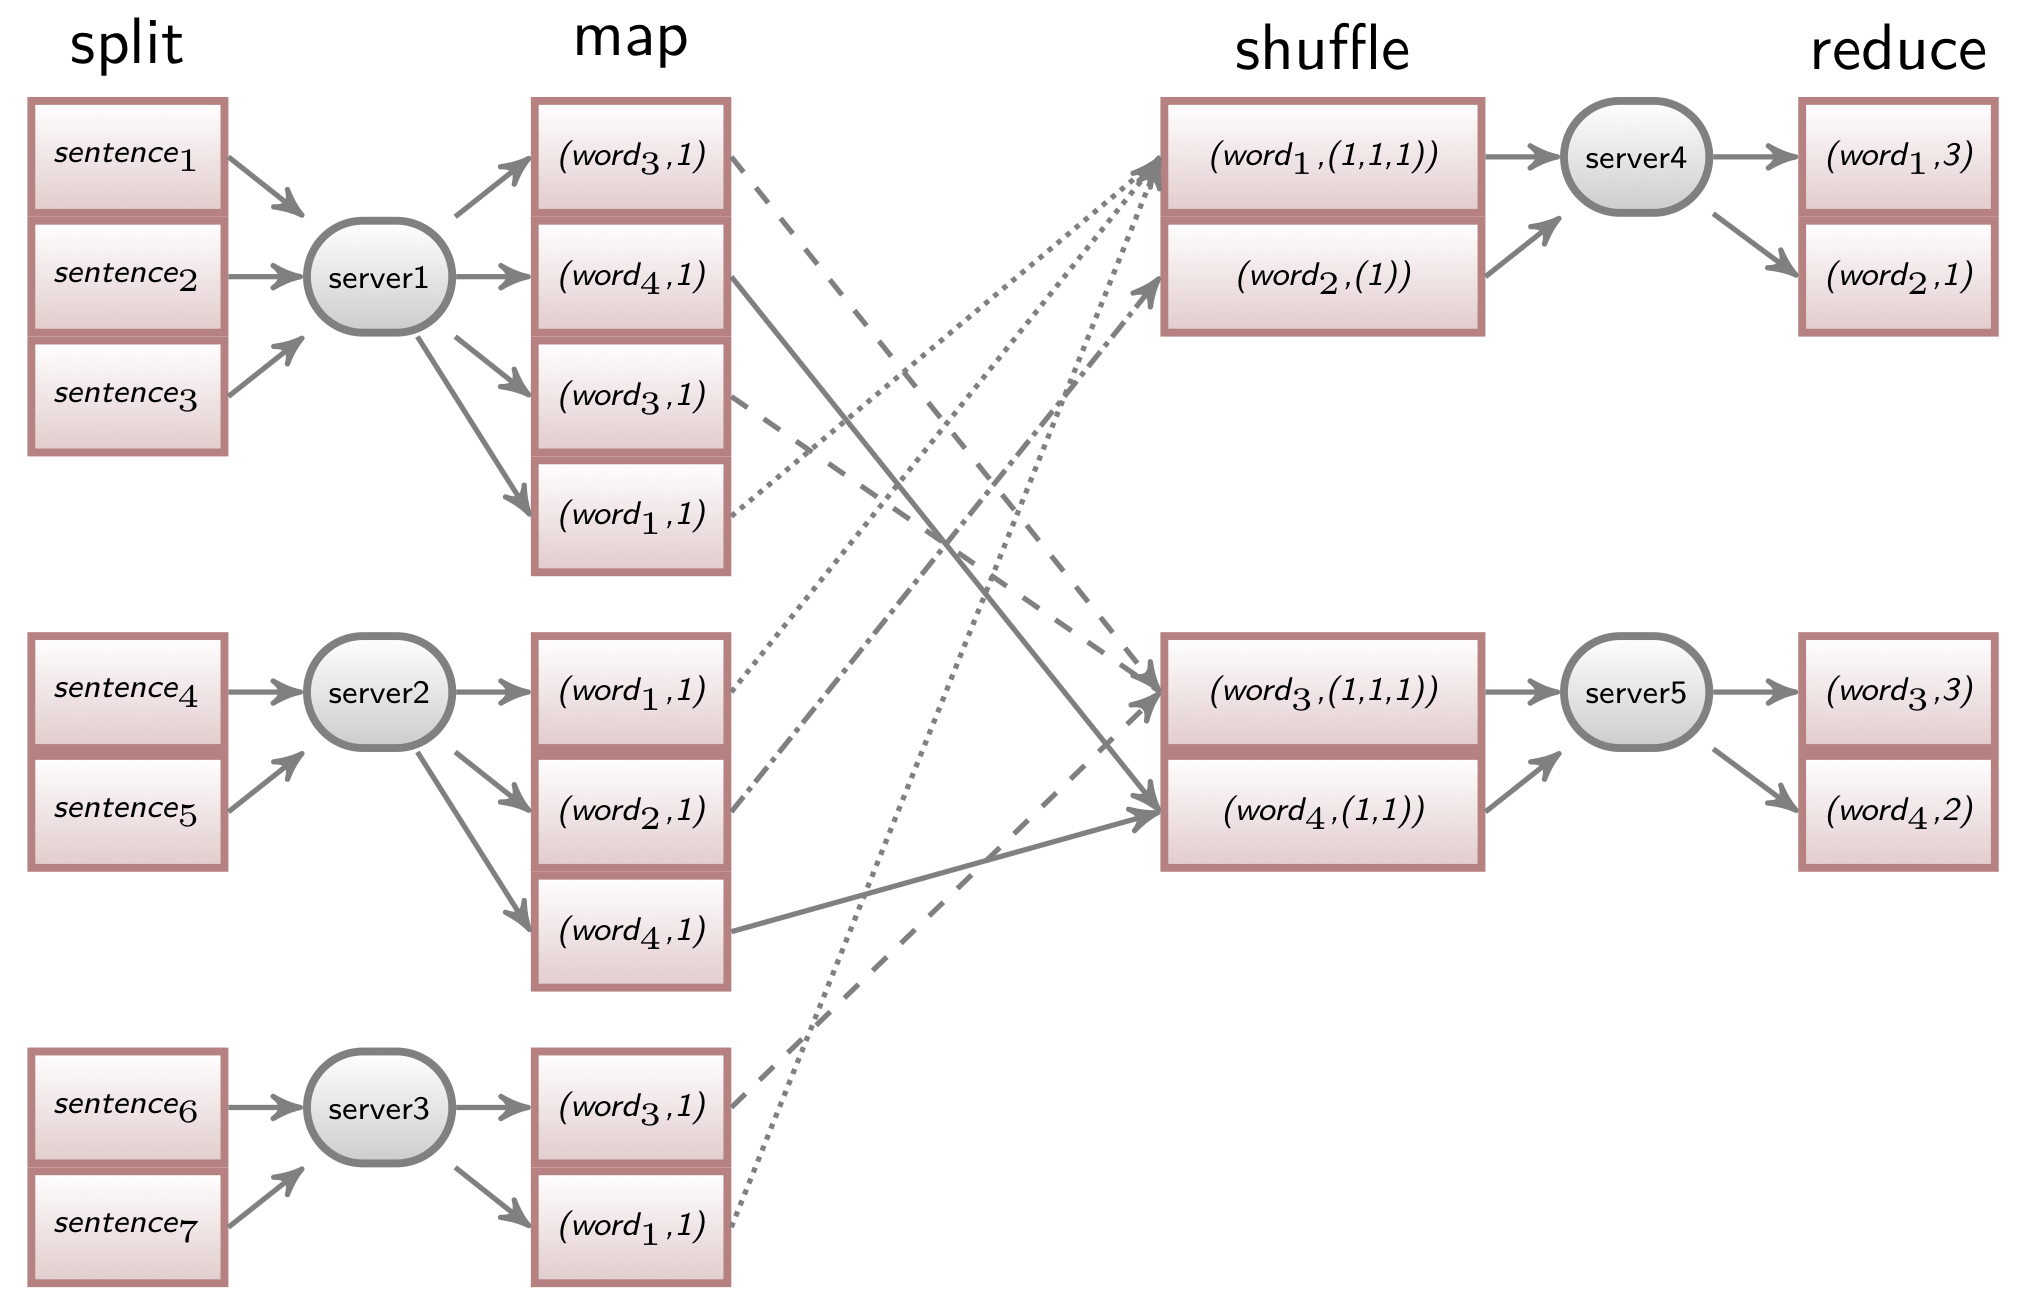
\includegraphics[width=0.70\linewidth]{images/AdvancedDataManagment/key_value_store/map_reduce.jpeg}
    \caption{Example of Map Reduce}
\end{figure}

\newpage
\begin{enumerate}
    \item \textbf{Split function} splits the document into sentences; each sentence is assigned to a worker process
    \item Worker thread starts a \textbf{map function} for each sentence. 
    \begin{itemize}
        \item It \textit{parses} a sentence and for \textit{each word} \(word_i\), the worker thread emits a \textit{key-value pair} \((word_i, 1)\) to indicate it encountered \(word_i\) once
        \item Intermediate result stored locally
    \end{itemize}
    \item In the \textbf{suffle phase} local intermediate results are read and grouped by words
    \begin{itemize}
        \item The 1-values for each word are concatenated into a list
        \item Key-value pair where the word \(word_i\) is the \textbf{key} and the \textbf{value} is a \textit{list of 1s} corresponding to individual occurrences of the word in all sentences
        \item Each word is assigned to a worker process
    \end{itemize}
    \item The \textbf{reduce function} calculates the total number of occurrences by \textit{summing the 1s}. The final results will look like a sequence of key-value pair \((word_i, sum_i)\)
\end{enumerate}

More formally:
\begin{itemize}
    \item \textbf{Split:} \textit{list ! list\((key_1, value_1)\)}:  split maps some input text to a list of key-value pairs
    \item \textbf{Map:} \((key_1, value_1)\) ! \(list(key_2, value_2)\): map processes one key-value pair and maps it to a list of key-value pairs
    \item \textbf{Shuffle:} \(list(key_2, value_2)\) ! (\(key_2\), \(list(value_2)\)): shuffle groups the individual key-value pairs by key and appends to each key a list that is a concatenation of the values of the individual pairs
    \item \textbf{Reduce:} (\(key_2, list(value_2)\)) ! (\(key_3, value_3\)): reduce aggregates a list of values into a single one
\end{itemize}

\subsubsection{Possible optimizations}
\begin{itemize}
    \item \textbf{Parallelization:} the map and as well as the reduce task can be run in parallel by different concurrent worker processes and even on multiple servers
    \item \textbf{Partitioning:} usually there are more reduce tasks to be executed than workers available. That is, each worker has to execute several reduce task on a set of different keys
    
    \newpage
    
    \item \textbf{Combination:} instead of locally storing lots of intermediate results of the map processes which later on have to be shuffled to other workers over the network. \textit{Combine} task can be run locally on each worker after the map phase, it  is similar to the reduce function as it groups the intermediate results by key and combines their values
    
    \begin{figure}[!hbp]
        \centering
        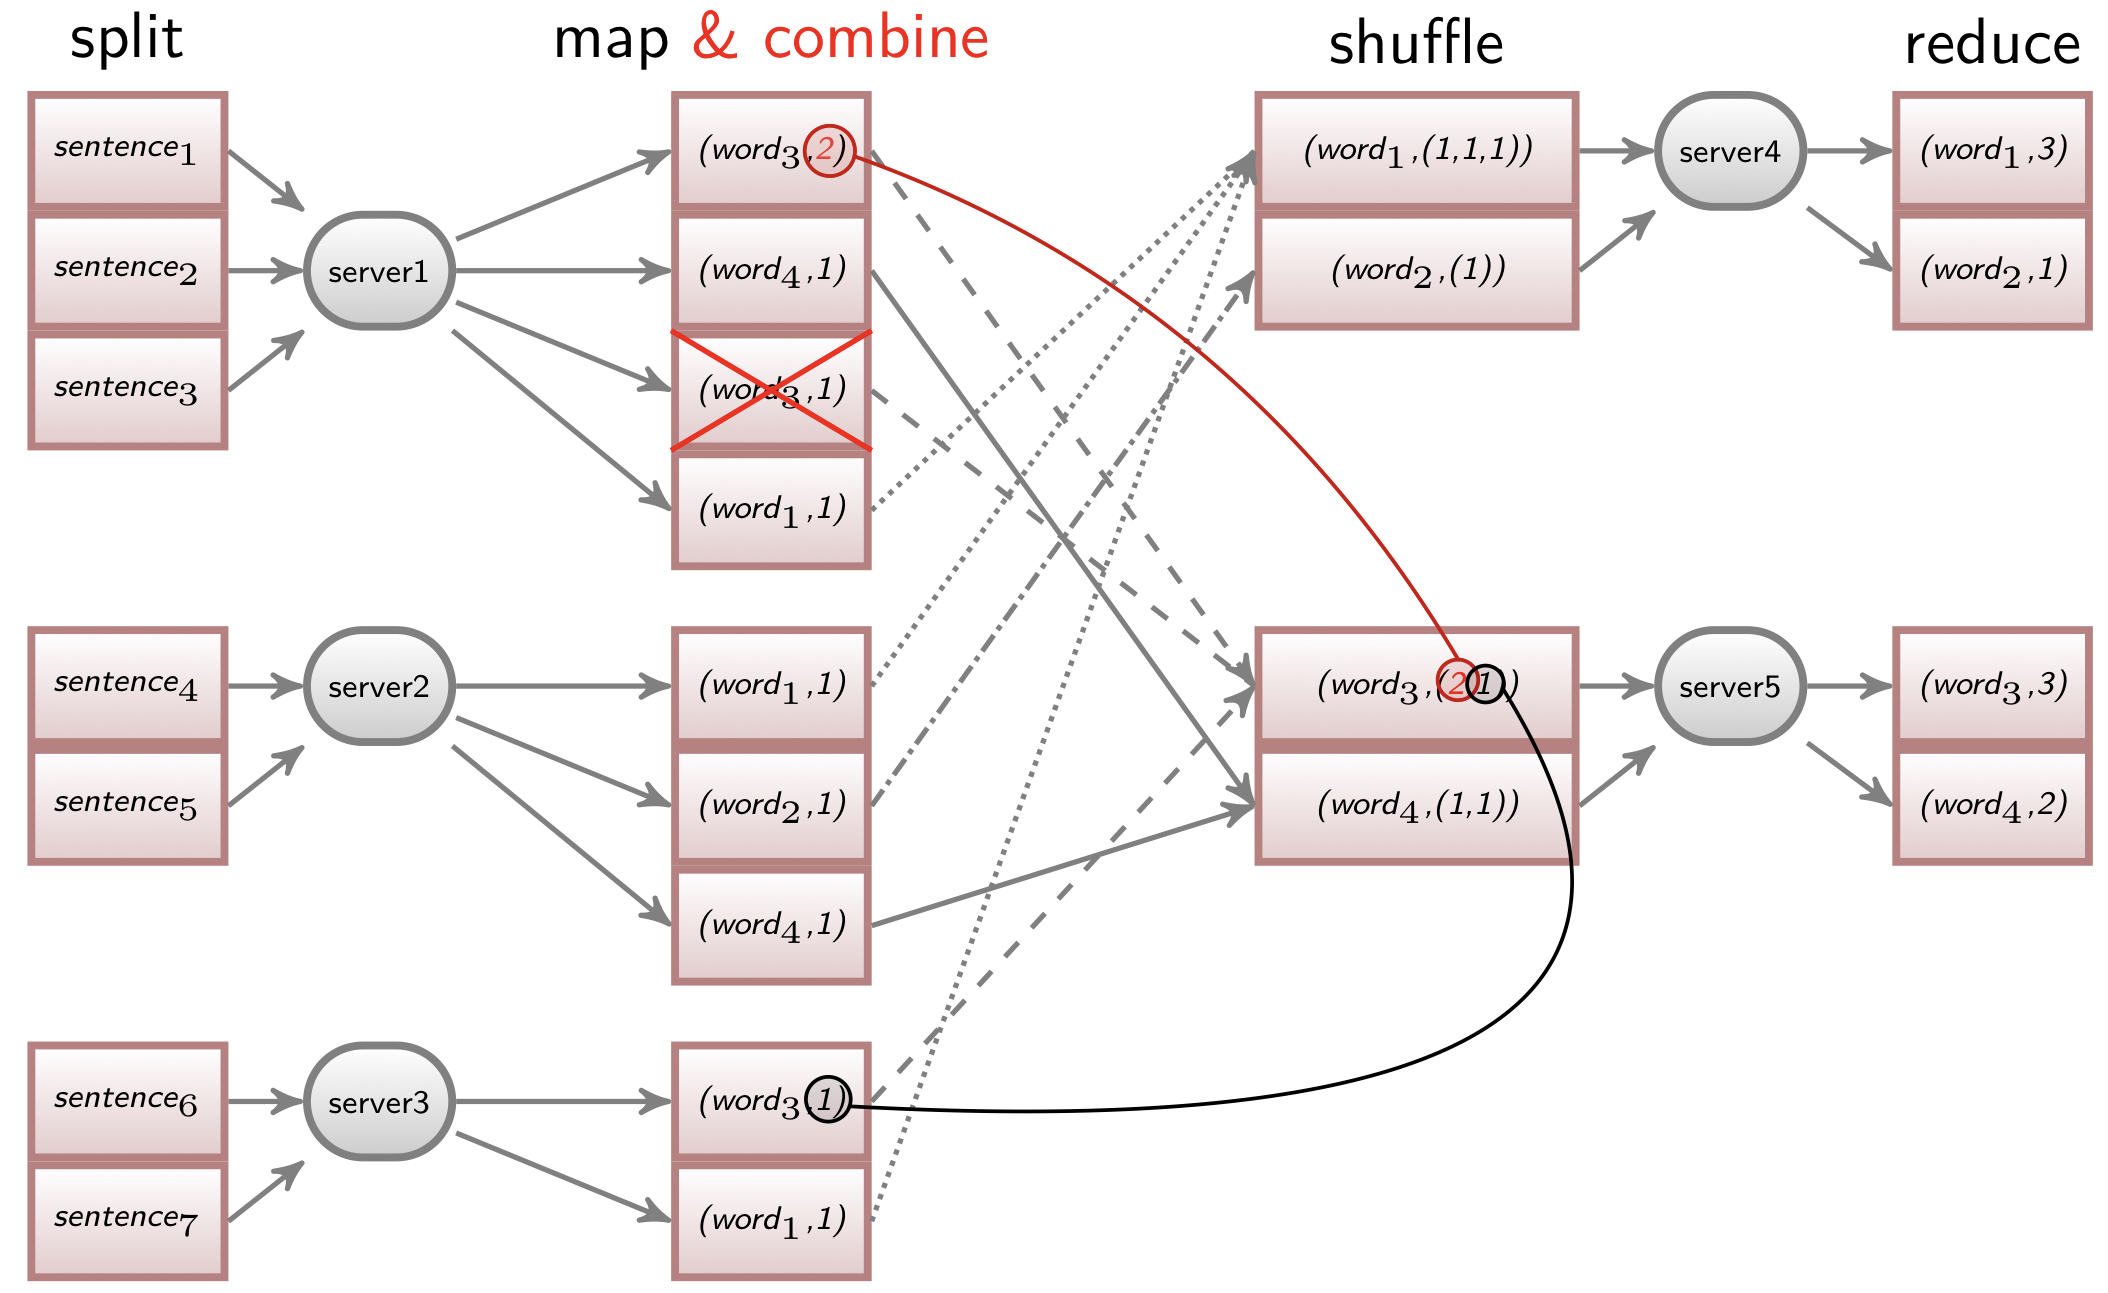
\includegraphics[width=0.70\linewidth]{images/AdvancedDataManagment/key_value_store/combination.jpeg}
        \caption{Example of Combination Map Reduce}
    \end{figure}
    
    \item \textbf{Data Locality:} transmitting data to a worker over the network is costly, thus the \textit{master} can take the location of data into account before assigning a task to a worker
    \item \textbf{Incremental Map-Reduce:} input data might be generated dynamically over a longer period of time. To improve evaluation of such data, the four steps can be interleaved and final results be obtained incrementally
\end{itemize}